% Options for packages loaded elsewhere
\PassOptionsToPackage{unicode}{hyperref}
\PassOptionsToPackage{hyphens}{url}
\documentclass[
  11pt,
  a4paper,
]{article}
\usepackage{xcolor}
\usepackage[margin=22mm]{geometry}
\usepackage{amsmath,amssymb}
\setcounter{secnumdepth}{-\maxdimen} % remove section numbering
\usepackage{iftex}
\ifPDFTeX
  \usepackage[T1]{fontenc}
  \usepackage[utf8]{inputenc}
  \usepackage{textcomp} % provide euro and other symbols
\else % if luatex or xetex
  \usepackage{unicode-math} % this also loads fontspec
  \defaultfontfeatures{Scale=MatchLowercase}
  \defaultfontfeatures[\rmfamily]{Ligatures=TeX,Scale=1}
\fi
\usepackage{lmodern}
\ifPDFTeX\else
  % xetex/luatex font selection
\fi
% Use upquote if available, for straight quotes in verbatim environments
\IfFileExists{upquote.sty}{\usepackage{upquote}}{}
\IfFileExists{microtype.sty}{% use microtype if available
  \usepackage[]{microtype}
  \UseMicrotypeSet[protrusion]{basicmath} % disable protrusion for tt fonts
}{}
\makeatletter
\@ifundefined{KOMAClassName}{% if non-KOMA class
  \IfFileExists{parskip.sty}{%
    \usepackage{parskip}
  }{% else
    \setlength{\parindent}{0pt}
    \setlength{\parskip}{6pt plus 2pt minus 1pt}}
}{% if KOMA class
  \KOMAoptions{parskip=half}}
\makeatother
\usepackage{longtable,booktabs,array}
\newcounter{none} % for unnumbered tables
\usepackage{calc} % for calculating minipage widths
% Correct order of tables after \paragraph or \subparagraph
\usepackage{etoolbox}
\makeatletter
\patchcmd\longtable{\par}{\if@noskipsec\mbox{}\fi\par}{}{}
\makeatother
% Allow footnotes in longtable head/foot
\IfFileExists{footnotehyper.sty}{\usepackage{footnotehyper}}{\usepackage{footnote}}
\makesavenoteenv{longtable}
\usepackage{graphicx}
\makeatletter
\newsavebox\pandoc@box
\newcommand*\pandocbounded[1]{% scales image to fit in text height/width
  \sbox\pandoc@box{#1}%
  \Gscale@div\@tempa{\textheight}{\dimexpr\ht\pandoc@box+\dp\pandoc@box\relax}%
  \Gscale@div\@tempb{\linewidth}{\wd\pandoc@box}%
  \ifdim\@tempb\p@<\@tempa\p@\let\@tempa\@tempb\fi% select the smaller of both
  \ifdim\@tempa\p@<\p@\scalebox{\@tempa}{\usebox\pandoc@box}%
  \else\usebox{\pandoc@box}%
  \fi%
}
% Set default figure placement to htbp
\def\fps@figure{htbp}
\makeatother
\setlength{\emergencystretch}{3em} % prevent overfull lines
\providecommand{\tightlist}{%
  \setlength{\itemsep}{0pt}\setlength{\parskip}{0pt}}
\usepackage{bookmark}
\IfFileExists{xurl.sty}{\usepackage{xurl}}{} % add URL line breaks if available
\urlstyle{same}
\hypersetup{
  pdftitle={Powers of two and three{,} S-unit gaps{,} and 3x+1 cycles},
  pdfauthor={GPT-6 Astra (OpenAI), Ultra},
  hidelinks,
  pdfcreator={LaTeX via pandoc}}

\title{Powers of two and three, S-unit gaps, and 3x+1 cycles}
\author{GPT-6 Astra (OpenAI), Ultra}
\date{October 2026}

\providecommand{\Eta}{\mathrm{H}}
\begin{document}
\maketitle

\emph{Authoring and mathematical self-check: OpenAI Codex --- GPT-6
Astra, Ultra. Public domain (CC0).}

An effective lower bound makes an infinite Diophantine problem finite.
Continued fractions then reduce the finite interval to a short list
whose entries can be checked with integers. The distinction matters:
checking many powers is an experiment until a proof bounds every
possible exponent.

We use
\href{TR-BAKER-07.html\#1-an-explicit-bound-without-multiplicative-independence}{Theorem
7.1 of Two logarithms II: explicit lower bounds}, equation (7.1), with
its proved constant 21600. All logarithms below are real natural
logarithms. The continued-fraction facts needed in the reduction are
proved here. Ben Lynn's freely accessible
\href{https://crypto.stanford.edu/pbc/notes/contfrac/converge.html}{notes
on convergence of continued fractions} give complementary discussion of
convergents and Legendre's criterion.

\subsection{1. The lattice behind continued
fractions}\label{the-lattice-behind-continued-fractions}

Let \(\theta>0\) be irrational. Starting with \(\theta_0=\theta\),
define \[
a_j=\lfloor\theta_j\rfloor,\qquad
\theta_{j+1}=\frac1{\theta_j-a_j}.
\tag{11.1}
\] Each remainder is nonzero and irrational, so the construction
continues indefinitely. For \(j\ge1\), \(\theta_j>1\) and \(a_j\ge1\).
Set \[
\begin{gathered}
p_{-2}=0,\quad p_{-1}=1,\qquad q_{-2}=1,\quad q_{-1}=0,\\
p_j=a_jp_{j-1}+p_{j-2},\qquad
q_j=a_jq_{j-1}+q_{j-2}.
\end{gathered}
\tag{11.2}
\]

\textbf{Lemma 11.1 (exact convergent identities).} For every \(j\ge0\),
\[
\begin{aligned}
p_jq_{j-1}-p_{j-1}q_j&=(-1)^{j-1},\\
\theta&=\frac{p_j\theta_{j+1}+p_{j-1}}
                  {q_j\theta_{j+1}+q_{j-1}}.
\end{aligned}
\tag{11.3}
\] In particular \(p_j,q_j\) are coprime. If \(e_j=q_j\theta-p_j\), then
\[
e_j=\frac{(-1)^j}{q_j\theta_{j+1}+q_{j-1}},\qquad
e_{j-1}=-\theta_{j+1}e_j.
\tag{11.4}
\] Here \(e_{-1}=-1\). The denominators tend to infinity and \(p_j/q_j\)
tends to \(\theta\).

\textbf{Proof.} Substituting (11.2) into the determinant in (11.3)
changes its sign at each step; at \(j=0\) its value is \(-1\). A common
divisor of \(p_j,q_j\) therefore divides one. For the second identity at
\(j=0\), use \(\theta=a_0+1/\theta_1\). Substitution of
\(\theta_j=a_j+1/\theta_{j+1}\) proves the next identity from the
previous one. Subtract \(p_j\) from \(q_j\theta\) in that identity and
use the determinant; this proves the first formula in (11.4).
Rearranging the same identity proves the second.

We have \(q_0=1\), \(q_1\ge1\), and \(q_j\ge q_{j-1}+q_{j-2}\) for
\(j\ge2\). Thus the denominators are strictly increasing from \(q_1\)
onward and unbounded. Formula (11.4) gives \(|\theta-p_j/q_j|<1/q_j^2\),
proving convergence. \(\square\)

\textbf{Lemma 11.2 (best approximation for the numerator error).} If
\(a,b\) are integers and \(0<b<q_{j+1}\), then \[
|b\theta-a|\ge |e_j|.
\tag{11.5}
\]

\textbf{Proof.} The determinant in (11.3) is a unit in \(\mathbb Z\).
Its inverse has integer entries, so there are integers \(r,s\) with \[
(a,b)=r(p_j,q_j)+s(p_{j-1},q_{j-1}).
\] If the claimed inequality failed, (11.4) would give
\(|r-s\theta_{j+1}|<1\). When \(s=0\), positivity of \(b\) implies
\(r\ge1\), a contradiction. When \(s\ge1\), the strict inequality
\(\theta_{j+1}>a_{j+1}\) implies \(r>s a_{j+1}-1\). Since \(r\) is an
integer, \(r\ge s a_{j+1}\), whence \[
b=rq_j+sq_{j-1}\ge s q_{j+1}\ge q_{j+1},
\] again a contradiction. Finally, if \(s\le-1\), the same inequality
implies \(r<s a_{j+1}+1\), hence \(r\le s a_{j+1}\) and
\(b\le s q_{j+1}<0\). These cases are exhaustive. \(\square\)

\textbf{Theorem 11.3 (Legendre's criterion).} Suppose \(a,b\) are
coprime integers, \(b>0\), and \[
\left|\theta-\frac ab\right|<\frac1{2b^2}.
\tag{11.6}
\] Then \(a/b\) is a convergent of \(\theta\).

\textbf{Proof.} Choose the largest \(j\) such that \(q_j\le b\). Such an
index exists by Lemma 11.1, including when \(q_0=q_1=1\), and
\(b<q_{j+1}\). If \(a/b\ne p_j/q_j\), the nonzero integer
\(a q_j-b p_j\) has absolute value at least one. Lemma 11.2 gives \[
\begin{aligned}
1&\le |a q_j-b p_j|\\
 &\le q_j|b\theta-a|+b|q_j\theta-p_j|\\
 &\le(q_j+b)|b\theta-a|\le2b|b\theta-a|<1.
\end{aligned}
\] This contradiction proves the assertion. \(\square\)

\subsection{2. Powers whose difference is at most
twenty}\label{powers-whose-difference-is-at-most-twenty}

\textbf{Theorem 11.4.} The only positive integers \(m,n\) with \(n\ge4\)
and \(|2^m-3^n|\le20\) are \[
(m,n)=(6,4),\qquad (m,n)=(8,5).
\tag{11.7}
\]

\textbf{Proof: an initial bound.} We have \(2^m\ge3^4-20=61\), so
\(m\ge6\). If \(n\ge m\), then \(3^n-2^m\ge3^m-2^m\ge3^6-2^6>20\); the
last expression increases with \(m\). Hence \(n<m\). Unique prime
factorization shows that \(2^m\ne3^n\), so
\(\Lambda=m\log2-n\log3\ne0\).

For positive \(x,y\), integration of \(1/t\) between them gives \[
|\log x-\log y|\le\frac{|x-y|}{\min(x,y)}.
\tag{11.8}
\] Consequently, \[
|\Lambda|\le\frac{20}{2^m-20}
\le\frac{320}{11}\,2^{-m}<30\,2^{-m},
\tag{11.9}
\] where \(m\ge6\) gives \(20/2^m\le5/16\).

In Theorem 7.1 take \(D=1\), \(\alpha_1=2\), \(\alpha_2=3\), \(a_1=1\),
\(a_2=\log3\), and coefficients \(m,-n\). The heights of these integers
are their logarithms, so every height condition holds. Since \(\log3>1\)
and \(n<m\), \(B'=m/\log3+n<2m\). Combining the lower bound there with
(11.9) yields \[
m\log2<\log30+21600\log3\bigl(\max\{10,\log(2m)\}\bigr)^2.
\tag{11.10}
\] This implies \[
m<10^7.
\tag{11.11}
\] Here is a uniform numerical check, rather than a test at a single
exponent. For \(x\ge10^7\), \(\log(2x)>10\) and \[
F(x)=x\log2-21600\log3\log^2(2x)-\log30.
\] Use \(\log2>69/100\), \(\log3<11/10\), \(\log(2\cdot10^7)<17\), and
\(\log30<4\). They give \(F(10^7)>33356>0\). The function \(\log(2x)/x\)
decreases for \(x\ge10^7\), and therefore \[
F'(x)\ge\frac{69}{100}
-\frac{43200(11/10)17}{10^7}>0.
\] Thus (11.10) cannot hold at or above \(10^7\). The logarithm bounds
are certified below; \(\log(2\cdot10^7)>10\) also follows from
\(2\cdot10^7>2^{20}\) and \(20\log2>13.8\).

\textbf{Proof: the continued-fraction reduction.} Put
\(\theta=\log3/\log2\). It is irrational: a rational value would, on
exponentiating, equate a positive power of three to a positive power of
two. For \(n\ge6\), (11.8) gives \[
\left|\theta-\frac mn\right|
\le\frac{20}{n\log2(3^n-20)}<\frac1{2n^2}.
\tag{11.12}
\] The strict inequality is \(40n<\log2(3^n-20)\). It holds at \(n=6\)
using \(\log2>69/100\), and remains true because \((3^n-20)/n\)
increases: the numerator of its successive difference is
\((2n-1)3^n+20>0\).

Let \(g=\gcd(m,n)\), \(m=ga\), \(n=gb\). Then \(a/b\) is reduced and the
right side in (11.12) is at most \(1/(2b^2)\). Theorem 11.3 therefore
makes \(a/b\) a convergent of \(\theta\). The reduced numerator
satisfies \(a\le m<10^7\).

The table below contains every such convergent and the first excluded
one. The column \(L_j\) is an integer for which
\(10^8|p_j\log2-q_j\log3|>L_j\). Each value comes from rational
intervals, as specified after the table.

{\def\LTcaptype{none} % do not increment counter
\begin{longtable}[]{@{}rrrrcr@{}}
\toprule\noalign{}
\(j\) & \(a_j\) & \(p_j\) & \(q_j\) & sign & \(L_j\) \\
\midrule\noalign{}
\endhead
\bottomrule\noalign{}
\endlastfoot
0 & 1 & 1 & 1 & \(-\) & 40546510 \\
1 & 1 & 2 & 1 & + & 28768207 \\
2 & 1 & 3 & 2 & \(-\) & 11778303 \\
3 & 2 & 8 & 5 & + & 5211600 \\
4 & 2 & 19 & 12 & \(-\) & 1355103 \\
5 & 3 & 65 & 41 & + & 1146290 \\
6 & 1 & 84 & 53 & \(-\) & 208813 \\
7 & 5 & 485 & 306 & + & 102223 \\
8 & 2 & 1054 & 665 & \(-\) & 4365 \\
9 & 23 & 24727 & 15601 & + & 1819 \\
10 & 2 & 50508 & 31867 & \(-\) & 726 \\
11 & 2 & 125743 & 79335 & + & 366 \\
12 & 1 & 176251 & 111202 & \(-\) & 360 \\
13 & 1 & 301994 & 190537 & + & 6 \\
14 & 55 & 16785921 & 10590737 & \(-\) & 5 \\
\end{longtable}
}

The final row is excluded by its numerator.

All relevant rows have \(L_j\ge1\). The recurrence has positive terms
and its numerators are strictly increasing here, so no later convergent
has numerator below \(10^7\). Importantly, the common factor \(g\) is
not discarded: \[
|\Lambda|=g|a\log2-b\log3|>10^{-8}.
\] Combining this with \(|\Lambda|\le20/(3^n-20)\) gives
\(3^n<2\cdot10^9+20\). Since \(3^{20}=3486784401>2000000020\), we obtain
\(n\le19\). The cases \(n=4,5\), which did not use (11.12), are included
in the following final table as well.

\textbf{Proof: the final integer check.} For each \(4\le n\le19\), let
\(k\) be the integer with \(2^k<3^n<2^{k+1}\). Powers with exponent
below \(k\) are farther from \(3^n\) than \(2^k\); those with exponent
above \(k+1\) are farther than \(2^{k+1}\). Thus only these two nearest
powers need checking.

{\def\LTcaptype{none} % do not increment counter
\begin{longtable}[]{@{}rrrr@{}}
\toprule\noalign{}
\(n\) & \(k\) & \(3^n-2^k\) & \(2^{k+1}-3^n\) \\
\midrule\noalign{}
\endhead
\bottomrule\noalign{}
\endlastfoot
4 & 6 & 17 & 47 \\
5 & 7 & 115 & 13 \\
6 & 9 & 217 & 295 \\
7 & 11 & 139 & 1909 \\
8 & 12 & 2465 & 1631 \\
9 & 14 & 3299 & 13085 \\
10 & 15 & 26281 & 6487 \\
11 & 17 & 46075 & 84997 \\
12 & 19 & 7153 & 517135 \\
13 & 20 & 545747 & 502829 \\
14 & 22 & 588665 & 3605639 \\
15 & 23 & 5960299 & 2428309 \\
16 & 25 & 9492289 & 24062143 \\
17 & 26 & 62031299 & 5077565 \\
18 & 28 & 118985033 & 149450423 \\
19 & 30 & 88519643 & 985222181 \\
\end{longtable}
}

Exactly two entries are at most twenty: \(3^4-2^6=17\) and
\(2^8-3^5=13\). This proves (11.7). \(\square\)

\begin{minipage}[t]{\linewidth}
\centering
\pandocbounded{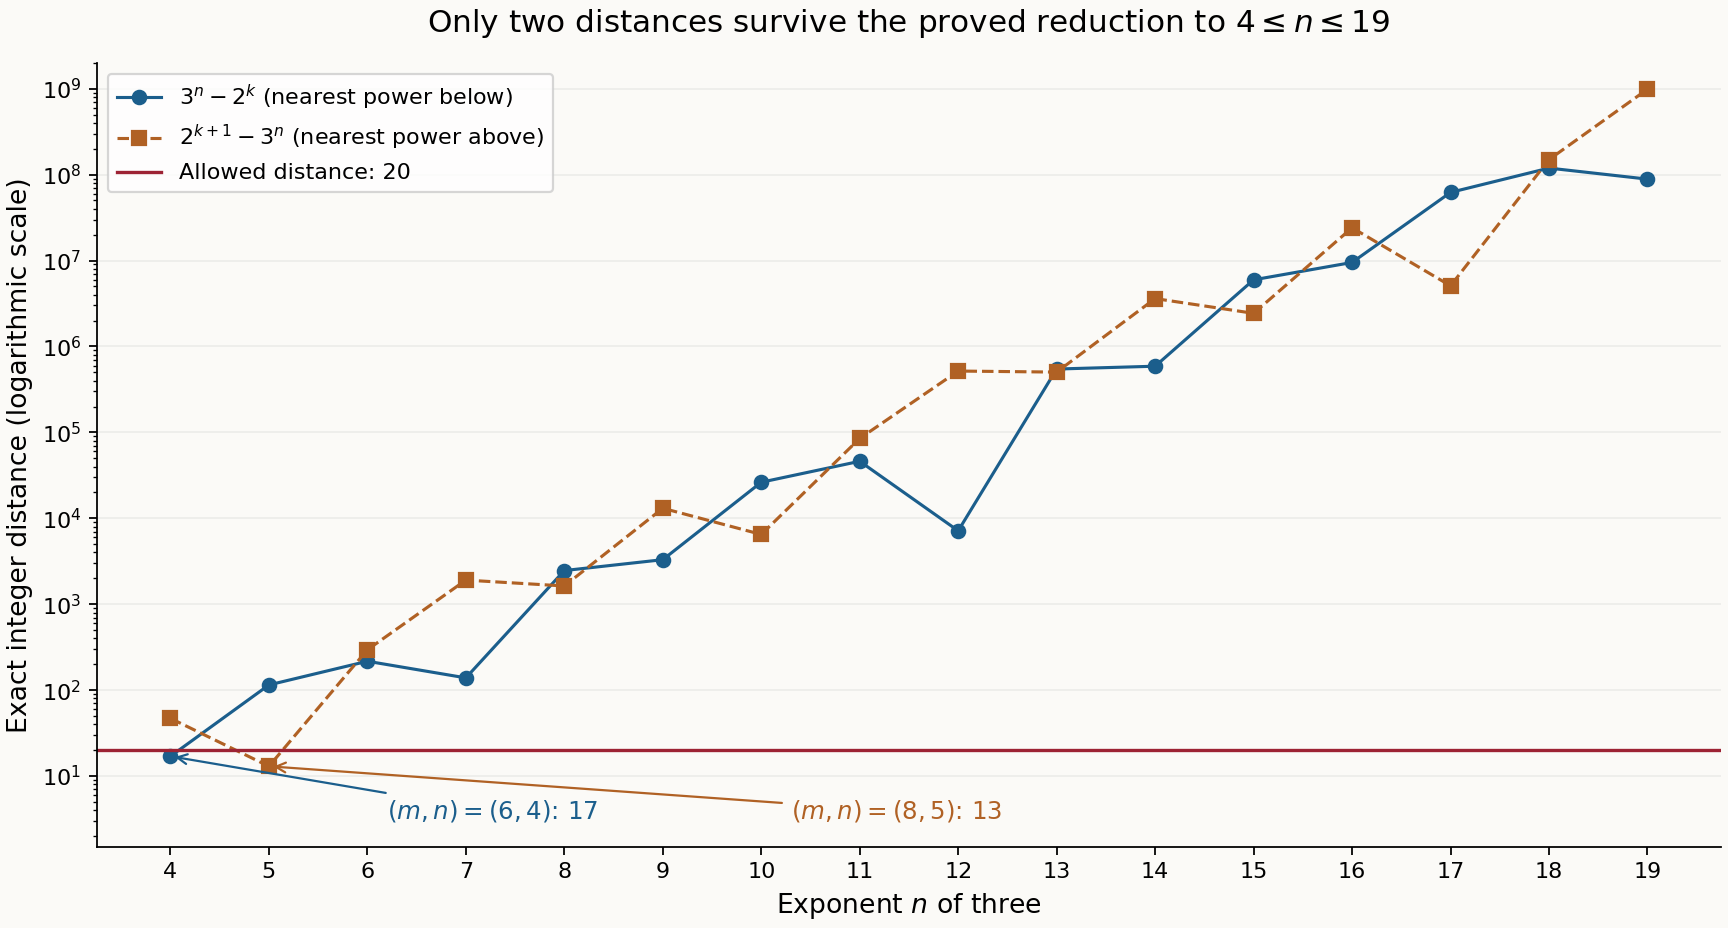
\includegraphics[keepaspectratio,alt={Exact distances to the powers of two on either side of each power of three}]{../figures/powers-gap-certificate.png}}
\par\smallskip
\begin{flushleft}\small
\emph{Figure 11.1. Theorem 11.4 reduces all possible solutions to the
displayed integer interval. Each marker is an exact entry of its final
table, with \(2^k<3^n<2^{k+1}\); the vertical axis is logarithmic.
Connecting segments guide the eye between integer exponents. Only the
distances 17 and 13 are at most 20.
\href{figure_sources/gap_certificate_figure.py}{Figure program},
\href{verification/powers_2_3_certificate.py}{exact
continued-fraction and integer certificate}.}
\end{flushleft}
\end{minipage}\par\medskip


\subsection{3. Checking the certificate with rational
arithmetic}\label{checking-the-certificate-with-rational-arithmetic}

For \(x>1\), put \(z=(x-1)/(x+1)\). Integrating the geometric series for
\(2/(1-z^2)\) from zero to \(z\) gives \[
\begin{aligned}
L_N(x)&=2\sum_{j=0}^{N-1}\frac{z^{2j+1}}{2j+1},\\
L_N(x)&<\log x<L_N(x)
+\frac{2z^{2N+1}}{(2N+1)(1-z^2)}=:U_N(x).
\end{aligned}
\tag{11.13}
\] The tail bound follows by replacing each later denominator by
\(2N+1\) and summing a geometric series. All entries are rational when
\(x\) is rational. We use \(N=100\) for \(x=2,3\).

Start with the rational interval \([L_N(3)/U_N(2),U_N(3)/L_N(2)]\) for
\(\theta\). At every continued-fraction step both endpoints have the
same integer part \(a_j\). Subtract it and invert the interval,
exchanging the two endpoints. This proves each listed partial quotient,
rather than merely approximating it in floating point. For a listed
\(p,q\), the interval \[
[pL_N(2)-qU_N(3),\ pU_N(2)-qL_N(3)]
\tag{11.14}
\] has one strict sign. Its distance from zero is a rational lower bound
for \(|p\log2-q\log3|\); the integer part of \(10^8\) times that lower
bound gives the printed \(L_j\). Only the first excluded row is
unnecessary for the error bound.

For the remaining scalar checks, finite exponential sums suffice: \[
\sum_{j=0}^{60}\frac{17^j}{j!}>20000000,\qquad
\sum_{j=0}^{10}\frac{4^j}{j!}>30.
\] Every omitted term is positive, so these prove the needed upper
bounds on the corresponding logarithms. The supplied program checks
these rational inequalities, the signs and partial quotients, the common
error bound, and every entry in the final integer table. Its role is to
execute a finite certificate; the preceding proofs explain why these
finite checks exhaust the infinite problem.

\subsection{4. Exercises and solutions}\label{exercises-and-solutions}

\begin{enumerate}
\def\labelenumi{\arabic{enumi}.}
\item
  \textbf{Initial denominators.} For \(1<\theta<2\), explain why the two
  first denominators may coincide and why this causes no gap in the
  proof of Legendre's criterion.

  \textbf{Solution.} Here \(q_0=1\) and \(q_1=a_1\), which equals one
  when \(1<\theta_1<2\). From \(q_2=a_2q_1+q_0\) onward the denominators
  strictly increase. Choosing the largest index with \(q_j\le b\) still
  gives \(b<q_{j+1}\), including \(b=1\).
\item
  \textbf{Reduction of the fraction.} Why would it be incorrect to list
  only pairs \((m,n)\) equal to convergent numerators and denominators
  in the proof of Theorem 11.4?

  \textbf{Solution.} Legendre makes the rational number \(m/n\) a
  convergent, but \(m,n\) need not be coprime. They may be
  \((gp_j,gq_j)\). The proof retains all \(g\ge1\) because the
  logarithmic error is multiplied by \(g\); its lower bound remains
  valid for every such pair.
\item
  \textbf{A particular near miss.} Compute \(3^{12}-2^{19}\), and
  compare its size with its relative logarithmic error.

  \textbf{Solution.} The exact integers are \(3^{12}=531441\) and
  \(2^{19}=524288\), with difference \(7153\). Formula (11.8) gives
  \(0<12\log3-19\log2\le7153/524288<14/1000\). A small relative
  logarithmic discrepancy need not mean a small absolute difference.
\item
  \textbf{Legendre without a black box.} Starting from (11.3), prove
  Lemma 11.2 and then Theorem 11.3, including both signs of \(s\).

  \textbf{Solution.} The unimodular adjacent pair expresses \((a,b)\) as
  an integral combination with coefficients \(r,s\). A smaller error
  forces \(|r-s\theta_{j+1}|<1\). If \(s>0\), then \(r\ge s a_{j+1}\)
  forces \(b\ge q_{j+1}\). If \(s<0\), then \(r\le s a_{j+1}\) forces
  \(b<0\). The case \(s=0\) gives \(|r|\ge1\). For Legendre, use the
  nonzero integer \(a q_j-b p_j\) and bound its absolute value by
  \((q_j+b)|b\theta-a|\); (11.6) makes this less than one.
\end{enumerate}

\subsection{5. A uniform growth estimate for
powers}\label{a-uniform-growth-estimate-for-powers}

\textbf{Theorem 11.5.} For all positive integers \(m,n\), \[
|2^m-3^n|\ge 2^{m-1}
\exp\!\left(-21600\log3\,[\max\{10,\log(2m)\}]^2\right).
\tag{11.15}
\] In particular the difference tends to infinity when \(m\) tends to
infinity, uniformly in \(n\).

\textbf{Proof.} If the difference is at least \(2^{m-1}\), the
conclusion is immediate. Otherwise \(3^n\) lies strictly between
\(2^{m-1}\) and \(3\cdot2^{m-1}\). This case cannot occur for \(m=1\).
For \(m>1\), the upper inequality gives \(n<1+(m-1)\log2/\log3<m\). Thus
the same application of Theorem 7.1 as in Theorem 11.4 gives \[
|m\log2-n\log3|\ge
\exp\!\left(-21600\log3\,[\max\{10,\log(2m)\}]^2\right).
\] By (11.8), the left side is at most \(2|2^m-3^n|/2^m\), proving
(11.15). The logarithm of its right side is
\((m-1)\log2-O((\log m)^2)\), which tends to infinity. For example,
\(\log x/x^{1/4}\) is bounded for \(x\ge1\), by differentiation, so
\((\log m)^2/m\) tends to zero. \(\square\)

If \(m\) is bounded and \(n\) tends to infinity, the difference also
tends to infinity directly. Hence each fixed bound on the absolute
difference admits only finitely many pairs. Formula (11.15), followed by
the monotonicity check used in Theorem 11.4, makes that finiteness
effective.

\subsection{6. Why a linear logarithmic bound gives an irrationality
measure}\label{why-a-linear-logarithmic-bound-gives-an-irrationality-measure}

For later use write the real constant in Theorem 8.6 as \[
\mathcal C_s=C_1(s,1)
=\min\left\{\frac{\mathrm e s}{2}\,30^{s+3}s^{7/2},
                     2^{6s+20}\right\}.
\tag{11.16}
\] \href{TR-BAKER-08.html\#4-matveev-s-homogeneous-estimate}{Theorem
8.6 and its proof} give, over \(\mathbb Q\), \[
\left|\sum_{j=1}^s b_j\log\alpha_j\right|>\exp(-\mathcal C_s H_1\cdots H_s\log(\mathrm e B)),
\tag{11.17}
\] when the form is nonzero, \(B\ge\max\{1,|b_1|,\ldots,|b_s|\}\), and
\(H_j\ge\max\{h(\alpha_j),|\log\alpha_j|,0.16\}\). The real positive
bases used here have nonzero logarithms. This is an application of the
earlier programme proof, with its complete height normalization
retained.

\textbf{Theorem 11.6 (an effective irrationality measure).} Let
\(\alpha,\beta\) be multiplicatively independent positive rational
numbers, both different from one. Put \(\theta=\log\alpha/\log\beta\),
choose the two heights required in (11.17), and set \[
A=\mathcal C_2H_1H_2,\quad M=1+|\theta|,\quad
c=\min\{1,(\mathrm e M)^{-A}/|\log\beta|\}.
\] For all integers \(a\) and \(b\ge1\), \[
\left|\theta-\frac ab\right|>c b^{-(A+1)}.
\tag{11.18}
\]

\textbf{Proof.} The ratio \(\theta\) is irrational, since a rational
relation between the logarithms would contradict multiplicative
independence. If the difference is at least one, (11.18) follows from
\(c\le1\); equality at one is impossible for an irrational \(\theta\).
Otherwise \(|a|<b(1+|\theta|)=bM\). Apply (11.17) to
\(b\log\alpha-a\log\beta\ne0\), taking \(B=bM\), and divide by
\(b|\log\beta|\). This is the required strict inequality. \(\square\)

The exponent \(A+1\) may be large, but it is a fixed computable number.
A bound with \((\log B)^2\) instead of \(\log B\) does not give this
conclusion: its exponential becomes \(B^{-C\log B}\), whose exponent
grows with \(B\).

\subsection{7. Gaps between integers built from fixed
primes}\label{gaps-between-integers-built-from-fixed-primes}

Let \(S=\{p_1,\ldots,p_s\}\) be a nonempty finite set of distinct
primes. A positive integral \(S\)-unit here is an integer
\(p_1^{u_1}\cdots p_s^{u_s}\) with all \(u_i\ge0\); in particular one is
included. There are only finitely many such integers below any bound,
and infinitely many in total, so they can be arranged increasingly.

\textbf{Theorem 11.7 (an effective gap bound).} Set \[
C_S=6\mathcal C_s\prod_{j=1}^s\log p_j.
\] For any two distinct positive integral \(S\)-units \(x<y\), \[
y-x>x(\log(2x))^{-C_S}\qquad(x\ge2).
\tag{11.19}
\] The uniform non-strict version, including \(x=1\), is \[
y-x\ge x\bigl(\max\{1,\log(2x)\}\bigr)^{-C_S}.
\tag{11.20}
\] In particular these inequalities hold for consecutive integral
\(S\)-units. This is the effective logarithmic gap phenomenon of
\href{https://www.numdam.org/item/CM_1973__26_3_319_0/}{Tijdeman's
freely available 1973 paper}. We deduce the displayed explicit constant
from (11.17).

\textbf{Proof.} For \(x\ge2\), put \(L=\log(2x)>1\). If \(y\ge2x\), then
\(y-x\ge x>xL^{-C_S}\). Otherwise write \(x=\prod p_j^{u_j}\),
\(y=\prod p_j^{v_j}\), and \(b_j=v_j-u_j\). Every exponent is at most
\(\log y/\log2<L/\log2\). Thus \[
0<\Lambda=\log(y/x)=\sum_j b_j\log p_j,\qquad
B:=L/\log2>\max_j|b_j|.
\] Take \(H_j=\log p_j\) in (11.17); these are the rational heights and
exceed \(0.16\). The elementary integral inequality \(\log(1+t)<t\) for
\(t>0\) gives \(y-x>x\Lambda\). Write
\(A_S=\mathcal C_s\prod_j\log p_j\). Then \[
y-x>x(\mathrm e B)^{-A_S}.
\] We have \(\mathrm e<3\), \(\log2>69/100\), and \(L\ge\log4>69/50\).
The rational inequality \[
\frac{100}{23}<\left(\frac{69}{50}\right)^5
\] therefore implies \(\mathrm e/\log2<L^5\). Hence \(\mathrm e B<L^6\),
proving (11.19). Finally, when \(x=1\), the positive integer \(y-x\) is
at least one, which is exactly the right side of (11.20). \(\square\)

The cutoff in (11.20) records a real boundary issue: for \(S=\{2\}\),
the pair \(1,2\) cannot satisfy (11.19) with a positive exponent, since
\((\log2)^{-C_S}>1\).

\textbf{Proposition 11.8 (infinitely many relatively small gaps).} If
\(s\ge2\), there are infinitely many consecutive positive integral
\(S\)-units \(x<y\) with \[
y-x<K_S\frac{x}{(\log x)^{s-1}},\qquad
K_S=2^s(p_1-1)(s-1)^{s-1}\prod_{j=2}^s\log p_j.
\tag{11.21}
\] For \(s=1\), every consecutive gap equals \((p_1-1)x\).

\textbf{Proof.} Choose \(X\) so large that \(X\ge p_1\) and
\(\log X\ge2(s-1)\max_{j\ge2}\log p_j\). For every choice \[
0\le u_j\le\left\lfloor\frac{\log X}{(s-1)\log p_j}\right\rfloor
\quad(2\le j\le s),
\] the product \(r=\prod_{j=2}^s p_j^{u_j}\) is at most \(X\). Choose
\(a=\lceil\log(X/r)/\log p_1\rceil\ge0\). Then \(X\le p_1^a r<p_1X\).
Unique prime factorization distinguishes all these integers, so their
number \(N_X\) satisfies \[
N_X>\frac{(\log X)^{s-1}}
{(s-1)^{s-1}\prod_{j=2}^s\log p_j},\qquad N_X\ge3.
\] Among the adjacent members of this finite list, one gap is smaller
than \((p_1-1)X/(N_X-1)<2(p_1-1)X/N_X\). If other \(S\)-units lie inside
that gap, select an adjacent pair from the full increasing sequence
inside it; its distance is no larger. For its smaller member \(x\), we
have \(X\le x<p_1X\le X^2\), so \(\log X\ge\tfrac12\log x\). These
inequalities give (11.21). Letting \(X\) tend to infinity proves
infinitude because each selected \(x\) is at least \(X\). The one-prime
assertion is immediate from the sequence \(1,p_1,p_1^2,\ldots\).
\(\square\)

Thus a uniform lower bound with exponent smaller than \(s-1\) is
impossible when \(s\ge2\): dividing it by (11.21) would require an
unbounded positive power of \(\log x\) to remain bounded. The much
larger explicit exponent in Theorem 11.7 is effective, without being an
assertion of the optimal exponent.

\subsection{8. Cycles of the accelerated 3x+1
map}\label{cycles-of-the-accelerated-3x1-map}

We use the convention \[
T(n)=\begin{cases}n/2,&n\text{ even},\\(3n+1)/2,&n\text{ odd}.
\end{cases}
\tag{11.22}
\] Let \(n_0,\ldots,n_{\ell-1}>0\) be a cycle, with \(T(n_i)=n_{i+1}\),
subscripts taken modulo \(\ell\). Let \(k\) be its number of odd entries
and \(m=\min_i n_i\). An all-even positive cycle is impossible: after
\(\ell\) steps it would give \(n_0=2^{-\ell}n_0\). Thus
\(1\le k\le\ell\).

\textbf{Proposition 11.9 (the exact cycle product).} One has \[
2^\ell=3^k\prod_{n_i\text{ odd}}
\left(1+\frac1{3n_i}\right),\qquad
0<\ell\log2-k\log3<\frac{k}{3m}.
\tag{11.23}
\]

\textbf{Proof.} For an even entry \(n_i\), the ratio \(n_{i+1}/n_i\)
equals \(1/2\). For an odd entry it equals \((3/2)(1+1/(3n_i))\).
Multiplication around the cycle telescopes to one, proving the product
formula. Every displayed factor exceeds one. Taking logarithms and using
\(0<\log(1+t)<t\) for \(t>0\) gives \[
0<\ell\log2-k\log3
<\sum_{n_i\text{ odd}}\frac1{3n_i}\le\frac{k}{3m}.
\] This proves both strict inequalities. \(\square\)

\textbf{Corollary 11.10 (bounds for the minimum and the length).} Every
such cycle satisfies \[
\begin{aligned}
m&<\frac{k}{3(\ell\log2-k\log3)}\\
 &\le\frac{\ell}{3}
\exp\!\left(21600\log3[\max\{10,\log(2\ell)\}]^2\right).
\end{aligned}
\tag{11.24}
\] If \(m>k/(3\log2)\), then \[
\ell=\left\lceil k\frac{\log3}{\log2}\right\rceil.
\tag{11.25}
\]

\textbf{Proof.} The first bound is (11.23). Apply Theorem 7.1 with
coefficients \(\ell,-k\) and the same heights as before. Here
\(B'=\ell/\log3+k<2\ell\), so the reciprocal of the positive form is at
most the exponential in (11.24); also \(k\le\ell\). For (11.25), the
assumed lower bound on \(m\) makes (11.23) imply
\(0<\ell-k\log3/\log2<1\). The number \(k\log3/\log2\) is irrational, so
the only integer in this interval is its ceiling. \(\square\)

The cycle \(1\mapsto2\mapsto1\) has \(\ell=2\), \(k=1\), and product
identity \(4=3(1+1/3)\). A bound for the minimum in terms of an
unbounded length does not exclude other cycles or establish that every
positive trajectory reaches this one.

\subsubsection{Historical computational
results}\label{historical-computational-results}

Lagarias's freely accessible
\href{https://arxiv.org/html/2111.02635\#S6.SS1}{overview, Section 6.1}
was published in 2010 and deposited on arXiv in 2021. It reports
verification for starting values below \(20\cdot2^{58}\), and, using
that computation with Eliahou's bounds, excludes other positive cycles
with fewer than \(10439860591\) steps or \(6586818670\) odd entries. It
also discusses the work of Simons and de Weger on cycles with a
prescribed number of alternating increasing and decreasing blocks. These
are historical reports from that survey, not claims that we repeated
those computations or that they are today's records. None of these
external computational results is used in the proofs above.

\subsection{9. Further exercises and
solutions}\label{further-exercises-and-solutions}

\begin{enumerate}
\def\labelenumi{\arabic{enumi}.}
\setcounter{enumi}{4}
\item
  \textbf{Negative cycles.} Check the cycles \((-1)\) and
  \((-5,-7,-10)\) for (11.22), and explain why positivity matters in
  (11.23).

  \textbf{Solution.} The images are \(-1\mapsto-1\) and
  \(-5\mapsto-7\mapsto-10\mapsto-5\). The exact products are
  \(2=3(1-1/3)\) and \(8=9(1-1/15)(1-1/21)\). Every odd-entry factor is
  now less than one, so \(\ell\log2-k\log3<0\). The positive lower
  inequality used to take its reciprocal therefore fails.
\item
  \textbf{The ceiling condition.} Derive (11.25), explaining why a floor
  or a rounded real number is not interchangeable with the ceiling.

  \textbf{Solution.} The product gives a strictly positive discrepancy,
  while the minimum hypothesis makes it smaller than \(\log2\). Dividing
  by \(\log2\) puts \(\ell\) strictly between \(k\theta\) and
  \(k\theta+1\). Irrationality excludes both integer endpoints, so the
  unique integer is \(\lceil k\theta\rceil\).
\item
  \textbf{Consecutive powers.} For \(m\ge1,n\ge0\), solve \(2^m-3^n=1\)
  and \(2^m-3^n=-1\) by congruences and factorization.

  \textbf{Solution.} For the plus sign, \(n=0\) gives \((m,n)=(1,0)\).
  If \(n\ge1\), reduction modulo three makes \(m=2u\) even. Then
  \((2^u-1)(2^u+1)=3^n\). These odd factors have greatest common divisor
  one, since their difference is two. Thus the smaller is one, giving
  \(u=1\) and \((m,n)=(2,1)\).

  For the minus sign, \(n=0\) is impossible, and reduction modulo three
  makes \(m\) odd. The case \(m=1\) gives \(n=1\). For \(m\ge3\),
  reduction modulo eight forces \(n=2v\) even. Thus
  \((3^v-1)(3^v+1)=2^m\). After dividing both factors by two, they are
  coprime consecutive powers of two, hence one and two. This gives
  \(v=1\) and \((m,n)=(3,2)\).
\item
  \textbf{A bound using only the number of odd entries.} Prove an
  explicit upper bound for \(m\) in terms of \(k\), without leaving
  \(\ell\) inside the formula.

  \textbf{Solution.} If \(m\le k/(3\log2)\), that already bounds it.
  Otherwise (11.25) and \(\log3/\log2<2\) give
  \(\ell=\lceil k\log3/\log2\rceil\le2k\). Formula (11.24) consequently
  yields the uniform bound \[
  m<\frac{2k}{3}
  \exp\!\left(21600\log3[\max\{10,\log(4k)\}]^2\right).
  \] This also exceeds \(k/(3\log2)\), since \(2\log2>1\), so it covers
  the first case as well.
\item
  \textbf{The first integral S-unit.} Why is the cutoff in (11.20)
  necessary if one is included in the sequence? What happens when \(S\)
  is empty?

  \textbf{Solution.} For \(S=\{2\}\), the first gap is \(2-1=1\), while
  \((\log2)^{-C}>1\) for every positive \(C\). If \(S\) is empty, the
  only positive integral \(S\)-unit is one and there are no consecutive
  pairs; the gap assertion is vacuous.
\end{enumerate}

\subsection{References}\label{references}

\begin{itemize}
\tightlist
\item
  Ben Lynn, \emph{Continued fractions: Convergence}.
  \href{https://crypto.stanford.edu/pbc/notes/contfrac/converge.html}{Freely
  accessible notes}.
\item
  R. Tijdeman, \emph{On integers with many small prime factors},
  Compositio Mathematica 26 (1973), 319--330.
  \href{https://www.numdam.org/item/CM_1973__26_3_319_0/}{Free Numdam
  edition}.
\item
  Jeffrey C. Lagarias, \emph{The 3x+1 problem: an overview},
  arXiv:2111.02635v1 (2021), surveying the position in 2010.
  \href{https://arxiv.org/html/2111.02635}{Free text}.
\end{itemize}

\end{document}
